\subsection{Classifieur de convexité}
\subsubsection{Etat de l'art}
Ce classifieur est basé sur le rapport « Hand Gesture Recognition Using Kinect » de Heng Du et TszHang To de l’Université de Boston \cite{hengDuEtAl}.  Leurs travaux ont portés sur la reconnaissance de nombre de doigts à partir d’une image capturé à l’aide d’une caméra kinect et de la bibliothèque OpenCV. 

<<<<<<< HEAD
Ce classifieur est basé sur la publication « Hand Gesture Recognition Using Kinect » de Heng Du et TszHang To de l’Université de Boston.  Leurs travaux ont porté sur la reconnaissance du nombre de doigts à partir d’une image capturée à l’aide d’une caméra Kinect et de la bibliothèque OpenCV. 
=======
\subsubsection{Présentation}
>>>>>>> a28458ec8f3969685ca5bfe7ec7a3d5a8488568f

Le principe général de ce classifieur est de détecter les points de convexités et de concavités du contour de la main et ainsi, selon un raisonnement logique, calculer le nombre de doigts levés.

Dans le but de rajouter un classifieur ne nécessitant pas de base d’apprentissage et ainsi diversifier le nombre d’images, ainsi que la diversité d’approches pour détecter et reconnaître les signes statiques de la main, ce classifieur a été implémenté suivant les étapes suivantes :

\paragraph{Détection du contour de la main}
Une fois une sous-image de la main extraite de l’image d’origine puis segmentée, nous avons utilisé la fonction implémentée d’OpenCV findContours() afin de pouvoir ainsi dérouler l’algorithme uniquement sur le contour de la main, comme illustrée par la figure suivante:  (\autoref{fig:contours}).

\begin{figure}[htb!]
\centerline{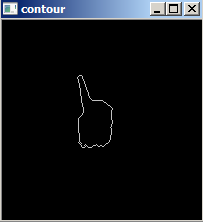
\includegraphics{contours.png}}
\caption{Contour de la main par findContours.}
\label{fig:contours}
\end{figure}

\paragraph{Approximation de la forme de la main par un polygone}
L’étape suivante permet de simplifier la détection des points de convexité et de concavité. Pour cela, on utilise la fonction implémentée d’OpenCV approxPolyDP() basée sur l’algorithme récursif de Ramer-Douglas-Peucker qui réduit le nombres de points d’une courbes en approximant une courbe similaire contenant moins de points, selon les étapes suivantes :

\begin{enumerate}
\item Traçage d’un segment entre le premier point de la courbe et le dernier.
\item Recherche du point le plus éloigné à ce segment et appartenant à la courbe et marquage de ce point comme visité.
\item Comparaison de distance entre ce point et le segment :
\begin{enumerate}
\item Si la distance est inférieure à $\alpha$ ($>0$ une valeur déterminée), alors on retire tous les points non marqués.
\item Si la distance est supérieure à $\alpha$, alors on marque le point et on trace le nouveau segment contenant le premier point et le dernier passant par le nouveau point marqué.
\end{enumerate}
\item On réapplique l’algorithme récursivement sur les deux segments : (premier point, nouveau point) et (nouveau point, dernier point), jusqu'à ce qu'on soit limité par le quadrillage pixellaire (deux points ont la même coordonnée dans l'image).
\item Une fois la récursion terminée, on retrace la nouvelle courbe avec les points visités uniquement.
\end{enumerate}

\paragraph{Détection des points convexes du polygone}
Afin de détecter les points de convexité de la main, on calcul un contour entourant le polygone en utilisant la fonction implémentée d’OpenCV convexHull(). Comme illustrée par la figure suivante: (\autoref{fig:convexePolygone}).

\begin{figure}[htb!]
\centerline{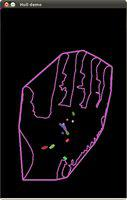
\includegraphics{convexePolygone.jpg}}
\caption{Polygone englobant de la main tel que claclulé par convexHull.}
\label{fig:convexePolygone}
\end{figure}

\paragraph{Détection des points de concavités du polygone}
En utilisant le résultat de la détection des points convexes, on effectue à présent la détection des points de concavité en utilisant une fonction adaptée d’OpenCV cvConvexityDefects(). Comme illustrée par la figure suivante : (\autoref{fig:convexityDefects}).

\begin{figure}[htb!]
\centerline{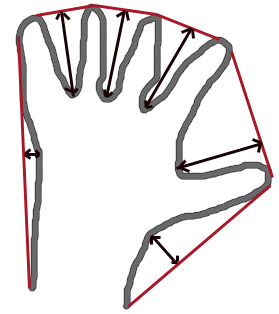
\includegraphics[scale=0.6]{convexityDefects.png}}
\caption{Points de concavité tels que détectés par cvConvexityDefects.}
\label{fig:convexityDefects}
\end{figure}

\paragraph{Filtrage des points de convexités et de concavités}
L’avant dernière étape de l’algorithme est l’étape la plus importante, car elle est assujettie à des paramètres statiques prédéterminés avant le lancement de cette dernière. 
Tout d’abord nous calculons un rectangle approximatif de la paume de la main en utilisant la fonction implémentée d’OpenCV minAreaRect().
Par la suite, afin de filtrer les points de convexité et respectivement de concavité, on compare leurs coordonnées en y avec le centre approximatif de la paume + $\epsilon$ ($>0$ valeur donnée) et respectivement $\beta$. Ces dernières nous permettent d’affiner nos résultats en augmentant la coordonnée en y du centre approximatif de la paume et ainsi réduire le nombre de points gardés.

Puis une fois les points de concavité et de convexité filtrés, on filtre une dernière fois les points de convexité selon leurs distances euclidiennes entre elles pour ainsi déterminer potentiellement le bout des doigts selon une distance minimale $\mu$.

\paragraph{Calcul du résultat du classifieur}
Enfin la dernière étape est un raisonnement logique selon le nombre de points trouvés. En effet le résultat du classifieur est donné par le nombre de points convexes identifiés :

\begin{itemize}
\item Si le nombre de points concaves $> 0$, Alors le résultat est le nombre de points convexes
\item Sinon, On regarde s’il existe un point convexe qui respecte la distance minimum entre le point de convexité et le centre de la paume:
\begin{itemize}
\item Alors le résultat est 1
\item Sinon le résultat est 0
\end{itemize}
\end{itemize}

\begin{figure}
\centerline{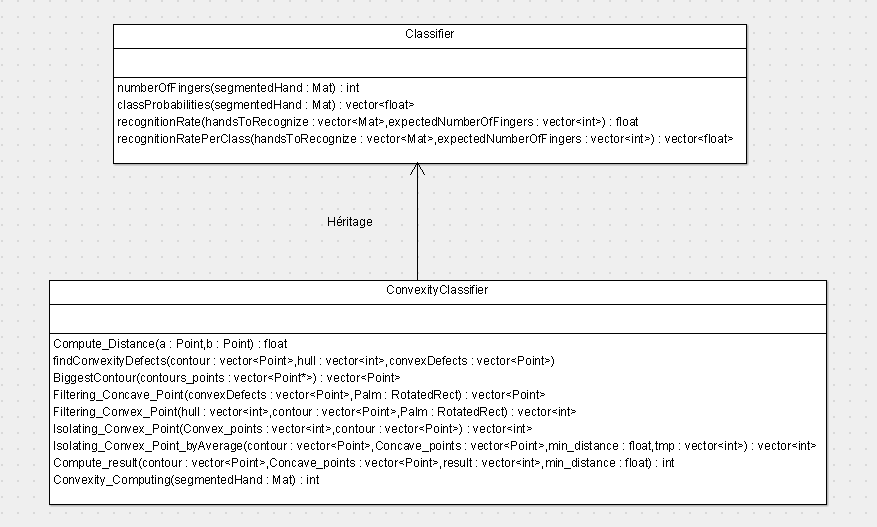
\includegraphics[scale=0.6]{umlConvexity.png}}
\caption{Diagramme UML du classifieur par convexités.}
\end{figure}

\subsubsection{Tests: paramètres optimaux}

Parce que les zones des images traitées sont différentes, 3 paramètres nécessitent d’être statiques car on ne peut prévoir à l’avance la direction de la main ni même sa distance par rapport à la caméra.
Dans ce principe, on a effectué une série d’essais pour déterminer des valeurs optimales pour les 3 paramètres :
\begin{itemize}
\item Distance minimale des points de convexités : $\epsilon$
\item Distance minimale des points de concavités : $\beta$
\item Distance minimale entre points de convexités : $\mu$
\end{itemize}

\begin{figure}[htb!]
\centerline{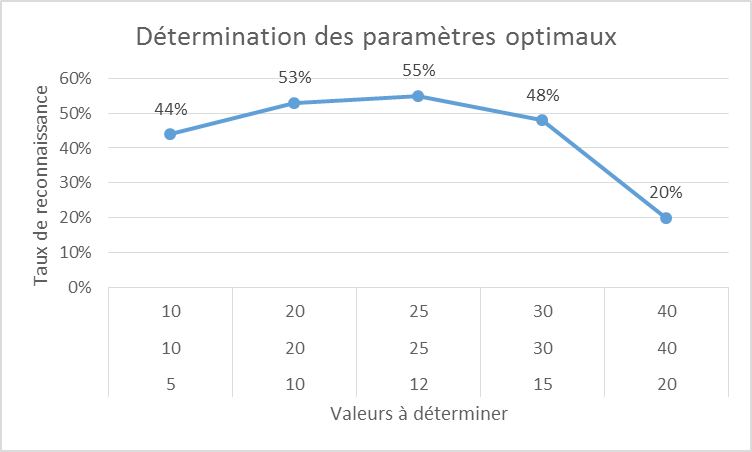
\includegraphics{convexiteParams.png}}
\caption{Taux de reconnaissance par rapport aux paramètres $\epsilon$, $\beta$ et $\mu$.}
\label{fig:convexiteParams}
\end{figure}

On remarque que le taux de reconnaissance atteint son maximum sur une plage de valeurs de [25, 25, 12 ] (\autoref{fig:convexiteParams}). 

A partir de ces tests préliminaires, on a peu réduire les intervalles de valeurs afin de déterminer les paramètres individuellement.

\paragraph{Détermination de la distance minimale des points de convexité}

\begin{figure}[htb!]
\centerline{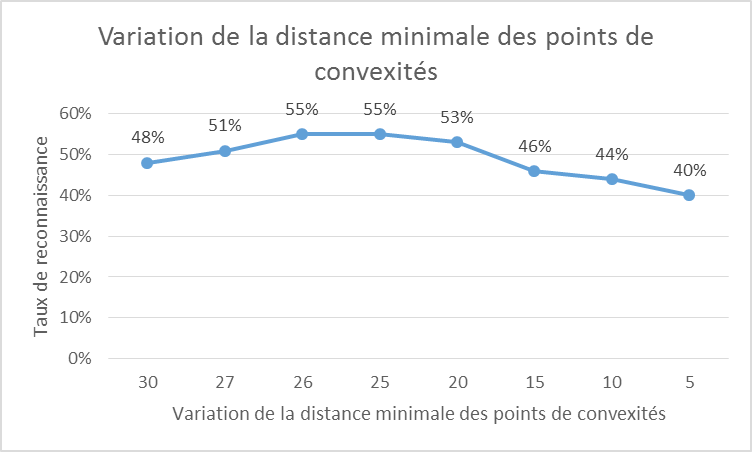
\includegraphics{convexiteDistMin.png}}
\caption{Taux de reconnaissance par rapport à la variation de distance minimale des points de convexité.}
\label{fig:convexiteDistMin}
\end{figure}

On remarque que le taux de reconnaissance s’améliore dans une fourchette de valeurs entre [ 27 , 20 ] et décroît en flèche en dehors de cet intervalle (\autoref{fig:convexiteDistMin}).

Cet intervalle représente la valeur moyenne d’écart entre le centre de la paume des mains dans la base d’apprentissage et les points de convexité, ce qui expliquerait ainsi cette amélioration du taux de reconnaissance. En dessous, les points de convexité à considérer seront trop importants et au dessus le nombre de points de convexité sera insuffisant pour pouvoir déterminer avec précision le résultat attendu.
On obtient alors une distance optimale de $\epsilon = 25$.

\paragraph{Détermination de la distance minimale des points de concavité}
\begin{figure}[htb!]
\centerline{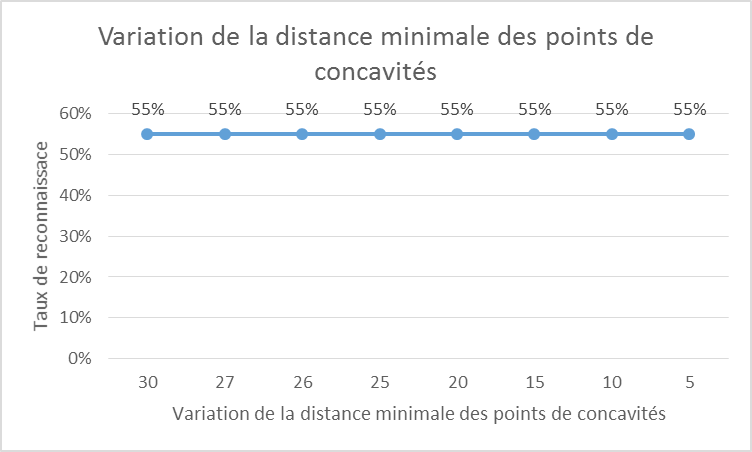
\includegraphics{concaviteDistMin.png}}
\caption{Taux de reconnaissance par rapport à la variation de distance minimale des points de concavité.}
\label{fig:concaviteDistMin}
\end{figure}

On remarque immédiatement, que le taux de reconnaissance est inchangé dans la variation de la distance minimale des points de concavité (\autoref{fig:concaviteDistMin}).

Ce résultat est expliqué par le fait que le calcul du résultat du classifieur est principalement basé sur le nombre de points convexes et non celui du nombre de points concaves. A partir de là, nous partons du principe que les deux distances peuvent prendre la même valeur : $\epsilon = \beta = 25$.

\paragraph{Détermination de la distance minimale entre points de convexités}
\begin{figure}[htb!]
\centerline{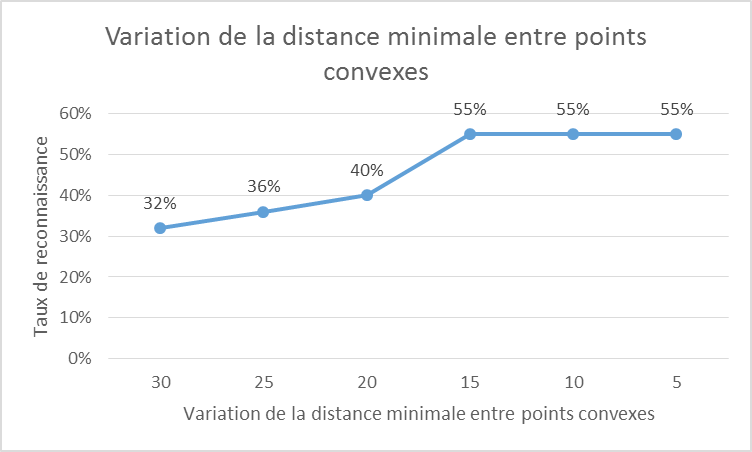
\includegraphics{convexiteEntreMin.png}}
\caption{Taux de reconnaissance par rapport à la variation de distance minimale entre points convexes.}
\label{fig:convexiteEntreMin}
\end{figure}

On remarque que le taux de reconnaissance s’accroît au fur et à mesure que la distance minimale diminue jusqu’à atteindre un maximum de 55\% à partir de la valeur 15. 

Ce résultat est expliqué par le fait que cette distance permet de détecter les doigts levés consécutifs de la main avec une distance moyenne entre 15 et 5. Cependant, cette distance ne permet pas de détecter efficacement les doigts levés éloignés comme pour faire des signes avec deux doigts éloignés. Par contre, elle permet de détecter efficacement les combinaisons de doigts au dessus de 2. 
De cette série de test, on déduit que la valeur intéressante de $\mu$ est 15, car elle permet de d’obtenir à la fois le meilleur taux mais aussi potentiellement une détection plus efficace pour les signes de la main contenant des combinaisons de doigts inférieurs à 2.

\subsubsection{Conclusion}
Avec les séries de test effectuées, on a pu atteindre un maximum de 55\% de taux de reconnaissance sur la base d’apprentissage sur laquelle l'ensemble des classifeurs s'est basé. De plus, ce classifieur ne nécessite pas de phase d’apprentissage. Il permet des calculs plus rapides et donc permettra à terme de pouvoir trancher les ambiguités lors de la combinaison de tous les classifieurs.

\subsubsection{Remarques}
Cependant, cet algorithme ne nous permet pas de dépasser un taux de reconnaissance au dessus de 55\%, car il a été admis sur des conditions d’acquisition restreintes, telles que :
\begin{itemize}
\item La détection d’une seule main à la fois
\item La main doit être à une distance constante par rapport à la caméra
\item La main doit être levée perpendiculairement au bras
\item Les doigts de la main doivent pointer (dans l’idéal vers le haut)
\item Les signes de la main doivent avoir uniquement les doigts levés de manière successive
\item Lors de la segementation, seule la main est sauvegardée (en dehors du poignet et tout autre forme parasite lors de l’acquisition).
\end{itemize}